\documentclass[tikz,border=2mm]{standalone}
\begin{document}
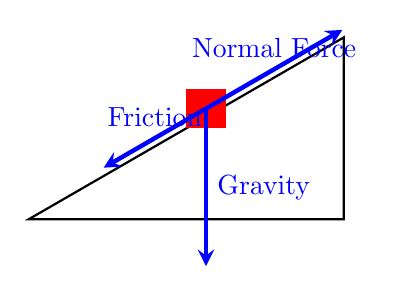
\begin{tikzpicture}

% Define the angle of inclination
\def\angle{30}

% Draw the inclined plane
\draw[thick] (0,0) -- (4,0) -- (4,{4*tan(\angle)}) -- cycle;

% Place the block on the inclined plane
\fill[red] (2,{2*tan(\angle)}) rectangle ++(0.5,0.5);

% Draw and label the force vectors
\begin{scope}[->,>=stealth,ultra thick,blue]
% Gravity
\draw (2.25,{2*tan(\angle)+0.25}) --++ (0,-2) node[midway,right] {Gravity};
% Normal force
\draw (2.25,{2*tan(\angle)+0.25}) --++ (\angle:2) node[midway,above] {Normal Force};
% Friction
\draw (2.25,{2*tan(\angle)+0.25}) --++ (180+\angle:1.5) node[midway,above] {Friction};
\end{scope}

\end{tikzpicture}
\end{document}